\section{Multi Instance Multi Label Learning}
 
\subsection*{Introduction}
\begin{frame}{Introduction to MIML}
	MIML problems combine motivations of multi instance and multi label ones.
	
	Given a set of labels $L = \{y_1, y_2,... y_l\}$
	$$D = \{(X_i, Y_i) | i \in [1, n]\}$$
	$$X_i = \{x_{i,k} | k \in [1, k_i], x_{i,k} \in \R^f\}$$
	$$Y_i = \{y_{i,h} | h \in [1, h_i], y_{i,h} \in L, h_i \leq l\}$$
	\begin{figure}[htbp]
		\centering
		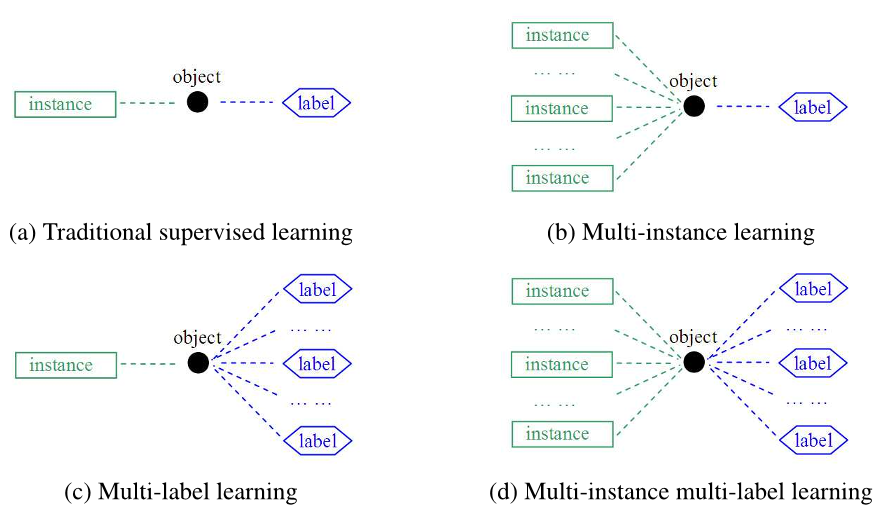
\includegraphics[scale = 0.20]{./images/confronto-miml.png}
		\caption{\textit{Different learning frameworks}}
	\end{figure}
	\begin{flushright}
		\cite{miml1}
	\end{flushright}
\end{frame}

\begin{frame}{SVM Solution}
	To allow regular SVMs to solve this problem, we use \textit{problem transformation}.
	
	There are 2 possibilities:
	\begin{itemize}
		\item MIML $\rightarrow$ MISL $\rightarrow$ SISL (used in this work)
		\item MIML $\rightarrow$ SIML $\rightarrow$ SISL
	\end{itemize}
	\begin{figure}[htbp]
		\centering
		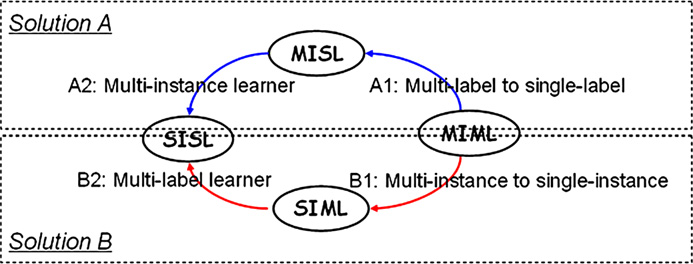
\includegraphics[scale = 0.40]{./images/2-metodi.png}
		\caption{\textit{Two possible solutions to implement MIML}}
	\end{figure}
\end{frame}

\begin{frame}{Multi label to single label}
	Excluding lossy approaches, the idea is to train a multi-instance (single label) classifier for each label.
	
	Given a MIML dataset $D = \{(X_i, Y_i) | i \in [1, n]\}$	we produce $l$ datasets as follows:
	$$D_{y_j} = \{(X_i, Y_{y_j}) | i \in [1, n]\} \ \forall j \in [1, l]$$
	Where
	$$Y_{y_j} = 
	\begin{cases}
		+1 \ if \ y_j \in Y_i \\
		-1 \ otherwise
	\end{cases}$$
	Then we train $L$ regular multi-instance SVMs and collect their results.
\end{frame}

\begin{frame}{Multi instance to single instance}

	Given one of MISL datasets produced at previous step, we compared the 3 methods previously exposed:
	\begin{itemize}
		\item SIL
		\item MI-SVM
		\item mi-SVM
	\end{itemize}
	
	They all use a standard SISL SVM as subroutine.
\end{frame}
